\documentclass[twoside,11pt]{homework}

\coursename{COMS W4705: Natural Language Processing (Fall 2018)} 

\studname{Wenbo Gao}    % YOUR NAME GOES HERE
\studmail{wg2313@columbia.edu}% YOUR UNI GOES HERE
\hwNo{4}                   % THE HOMEWORK NUMBER GOES HERE
\date{\today} % DATE GOES HERE

% Uncomment the next line if you want to use \includegraphics.
\usepackage{graphicx}
%\includegraphics[height=0.3\textheight]{hw0.pdf}
\usepackage{physics}
% \usepackage{tikz-cd}

% environments: theorem[*rename], proof[*rename], 

\begin{document}
\maketitle

\section*{Problem 1}

Using the raw co-occurence counts:
\begin{itemize}
\item Which word is the most similar to 'animal' using euclidean distance?

  'dog'.
  \[
    \text{dis}(\text{dog}, \text{animal})
    = \sqrt{(0-2)^2+(4-3)^2+(0-0)^2+(4-3)^2+(2-0)^2+(2-3)^2}
    = \sqrt{11}
  \]
  \[
    \text{dis}(\text{cat}, \text{animal})
    = \sqrt{(4-2)^2+(0-3)^2+(0-0)^2+(3-3)^2+(3-0)^2+(10-3)^2}
    = \sqrt{71}
  \]
  \[
    \text{dis}(\text{computer}, \text{animal})
    = \sqrt{(0-2)^2+(0-3)^2+(0-0)^2+(5-3)^2+(0-0)^2+(5-3)^2}
    = \sqrt{21}
  \]
  \[
    \text{dis}(\text{run}, \text{animal})
    = \sqrt{(4-2)^2+(3-3)^2+(5-0)^2+(0-3)^2+(3-0)^2+(4-3)^2}
    = 4 \sqrt{3}
  \]
  \[
    \text{dis}(\text{mouse}, \text{animal})
    = \sqrt{(2-2)^2+(10-3)^2+(5-0)^2+(4-3)^2+(3-0)^2+(0-3)^2}
    = \sqrt{93}
  \]
\item Which word is the most similar to 'animal' using cosine similarity?

  'run'.
  \[
  \begin{aligned}
  \text{dis}(\text{dog}, \text{animal})
  &= \frac{\vec{v}_{dog} \cdot \vec{v}_{animal}}{||\vec{v}_{dog}|| \ ||\vec{v}_{animal}||}\\
  &= \frac{0*2 + 4*3 + 0*0 + 4*3 + 2*0 + 2*3}{ \sqrt{0^2+4^2+0^2+4^2+2^2+2^2}
    \sqrt{2^2+3^2+0^2+3^2+0^2+3^2}}\\
  &= 0.851942751369
  \end{aligned}
  \]

  \[
  \begin{aligned}
  \text{dis}(\text{cat}, \text{animal})
  &= \frac{\vec{v}_{cat} \cdot \vec{v}_{animal}}{||\vec{v}_{cat}|| \ ||\vec{v}_{animal}||}\\
  &= \frac{4*2 + 0*3 + 0*0 + 3*3 + 3*0 + 10*3}{ \sqrt{4^2+0^2+0^2+3^2+3^2+10^2}
    \sqrt{2^2+3^2+0^2+3^2+0^2+3^2}}\\
  &= 0.729230142593
  \end{aligned}
  \]

  \[
  \begin{aligned}
  \text{dis}(\text{computer}, \text{animal})
  &= \frac{\vec{v}_{computer} \cdot \vec{v}_{animal}}{||\vec{v}_{computer}|| \ ||\vec{v}_{animal}||}\\
  &= \frac{0*2 + 0*3 + 0*0 + 5*3 + 0*0 + 5*3}{ \sqrt{0^2+0^2+0^2+5^2+0^2+5^2}
    \sqrt{2^2+3^2+0^2+3^2+0^2+3^2}}\\
  &= 0.762000762
  \end{aligned}
  \]

  \[
  \begin{aligned}
  \text{dis}(\text{run}, \text{animal})
  &= \frac{\vec{v}_{run} \cdot \vec{v}_{animal}}{||\vec{v}_{run}|| \ ||\vec{v}_{animal}||}\\
  &= \frac{4*2 + 3*3 + 5*0 + 0*3 + 3*0 + 4*3}{ \sqrt{4^2+3^2+5^2+0^2+3^2+4^2}
    \sqrt{2^2+3^2+0^2+3^2+0^2+3^2}}\\
  &= 0.601431982944 
  \end{aligned}
  \]

  \[
  \begin{aligned}
  \text{dis}(\text{mouse}, \text{animal})
  &= \frac{\vec{v}_{mouse} \cdot \vec{v}_{animal}}{||\vec{v}_{mouse}|| \ ||\vec{v}_{animal}||}\\
  &= \frac{2*2 + 10*3 + 5*0 + 4*3 + 3*0 + 0*3}{ \sqrt{2^2+10^2+5^2+4^2+3^2+0^2}
    \sqrt{2^2+3^2+0^2+3^2+0^2+3^2}}\\
  &= 0.665758353436 
  \end{aligned}
  \]

\end{itemize}

\section*{Problem 2}
To determine if two senses of a lemma are homonyms or polysemy
\begin{itemize}
\item If there exists a subset of lemmas (with stop words removed) that coexists
  in both synsets or hyponyms of both synsets, then they are homonyms;
\item Otherwise, polysemy.
\end{itemize}

\section*{Problem 3}
\subsection*{a)}
  \begin{figure}[h]
  	\centering
  	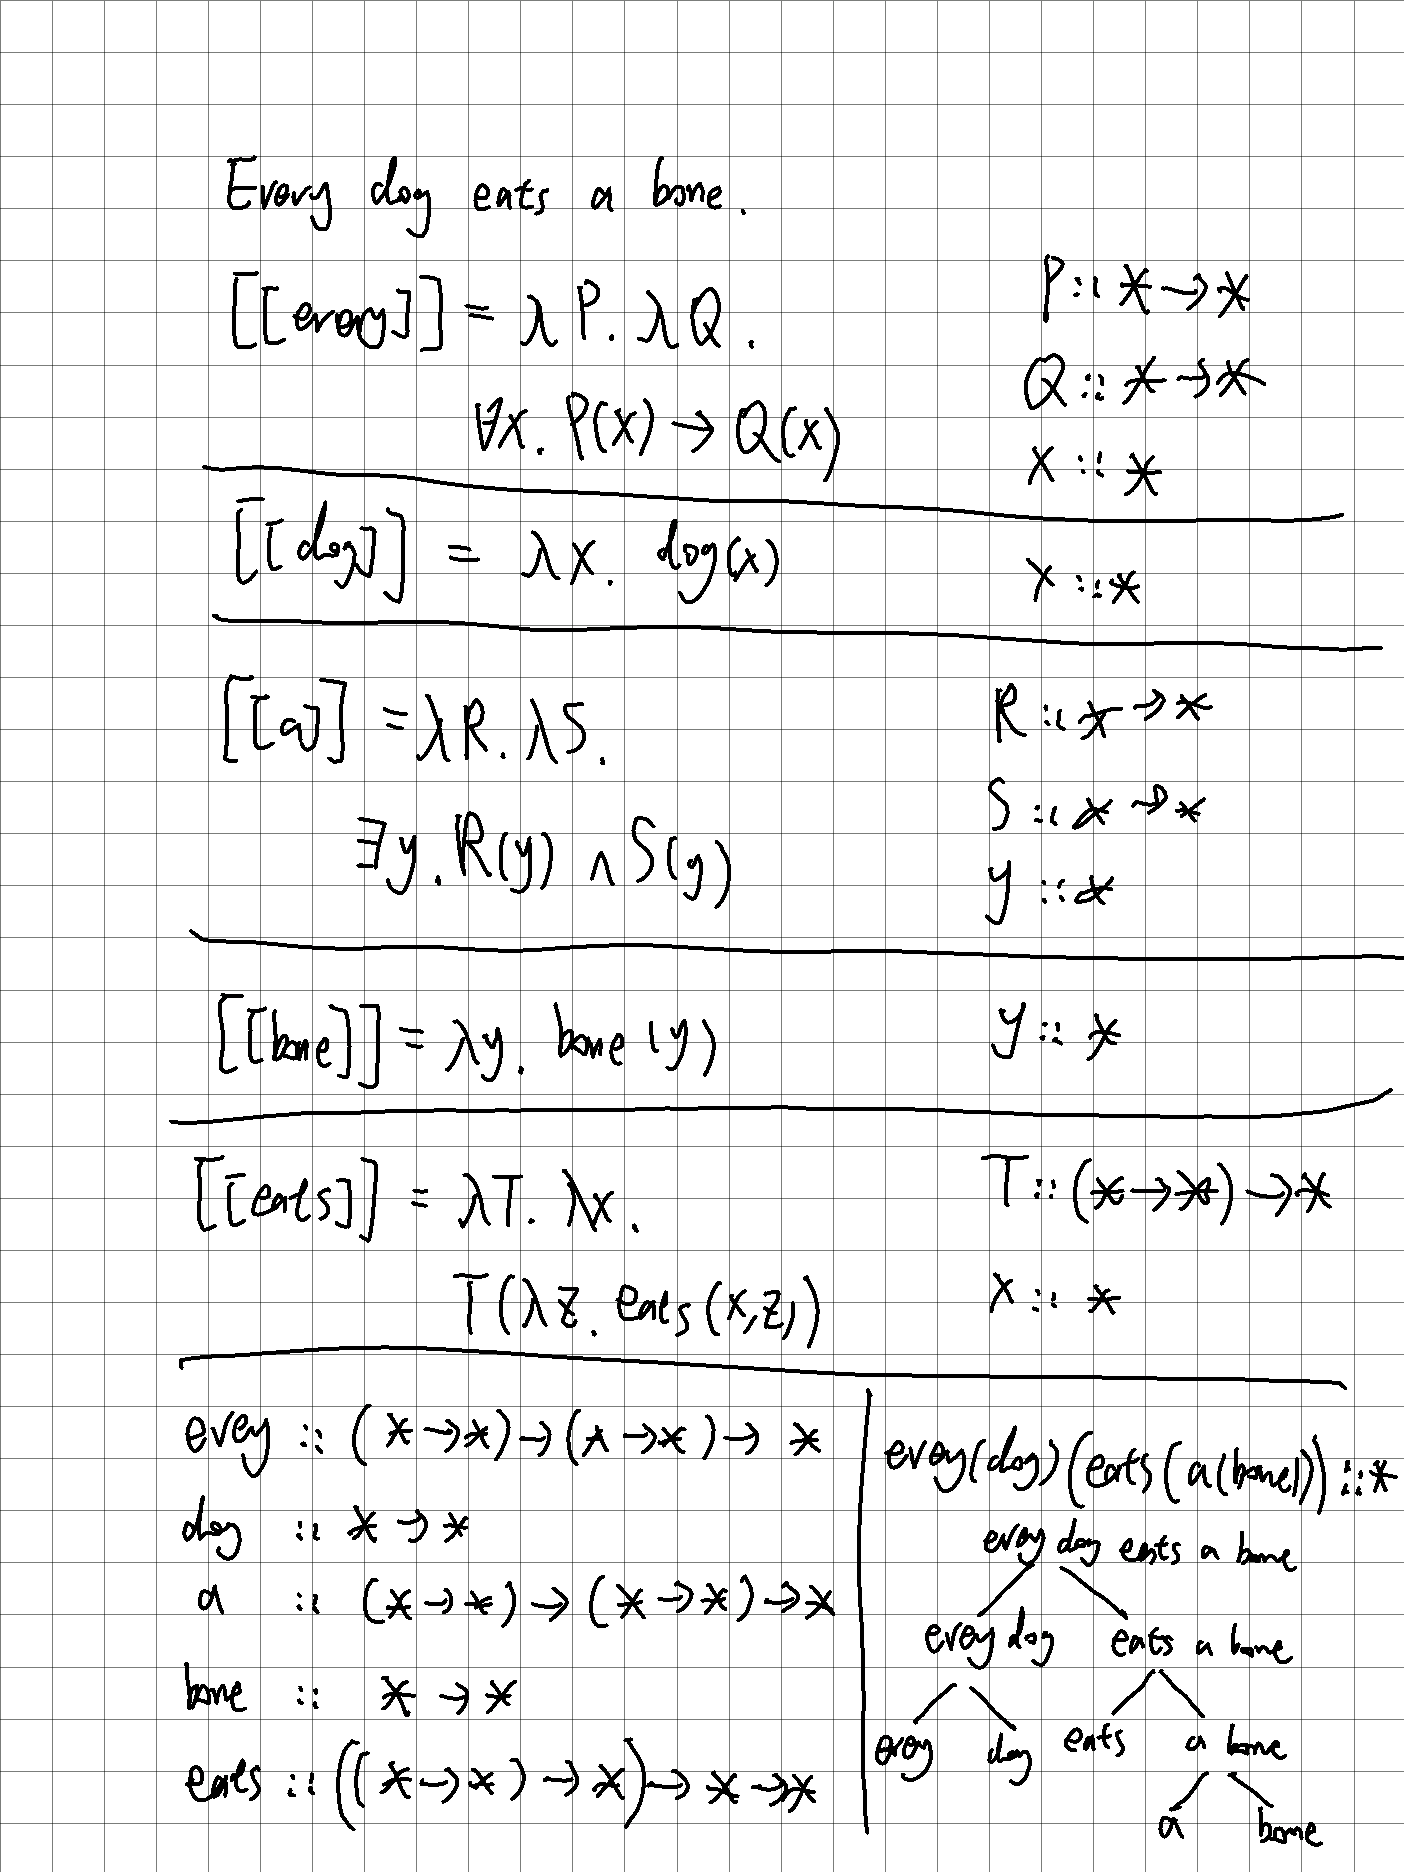
\includegraphics[width=0.7\linewidth]{../parse_tree}
  	\caption{problem 3 (a)}
  	\label{fig:01}
  \end{figure}

\subsection*{b)}
  \begin{figure}[h]
  	\centering
  	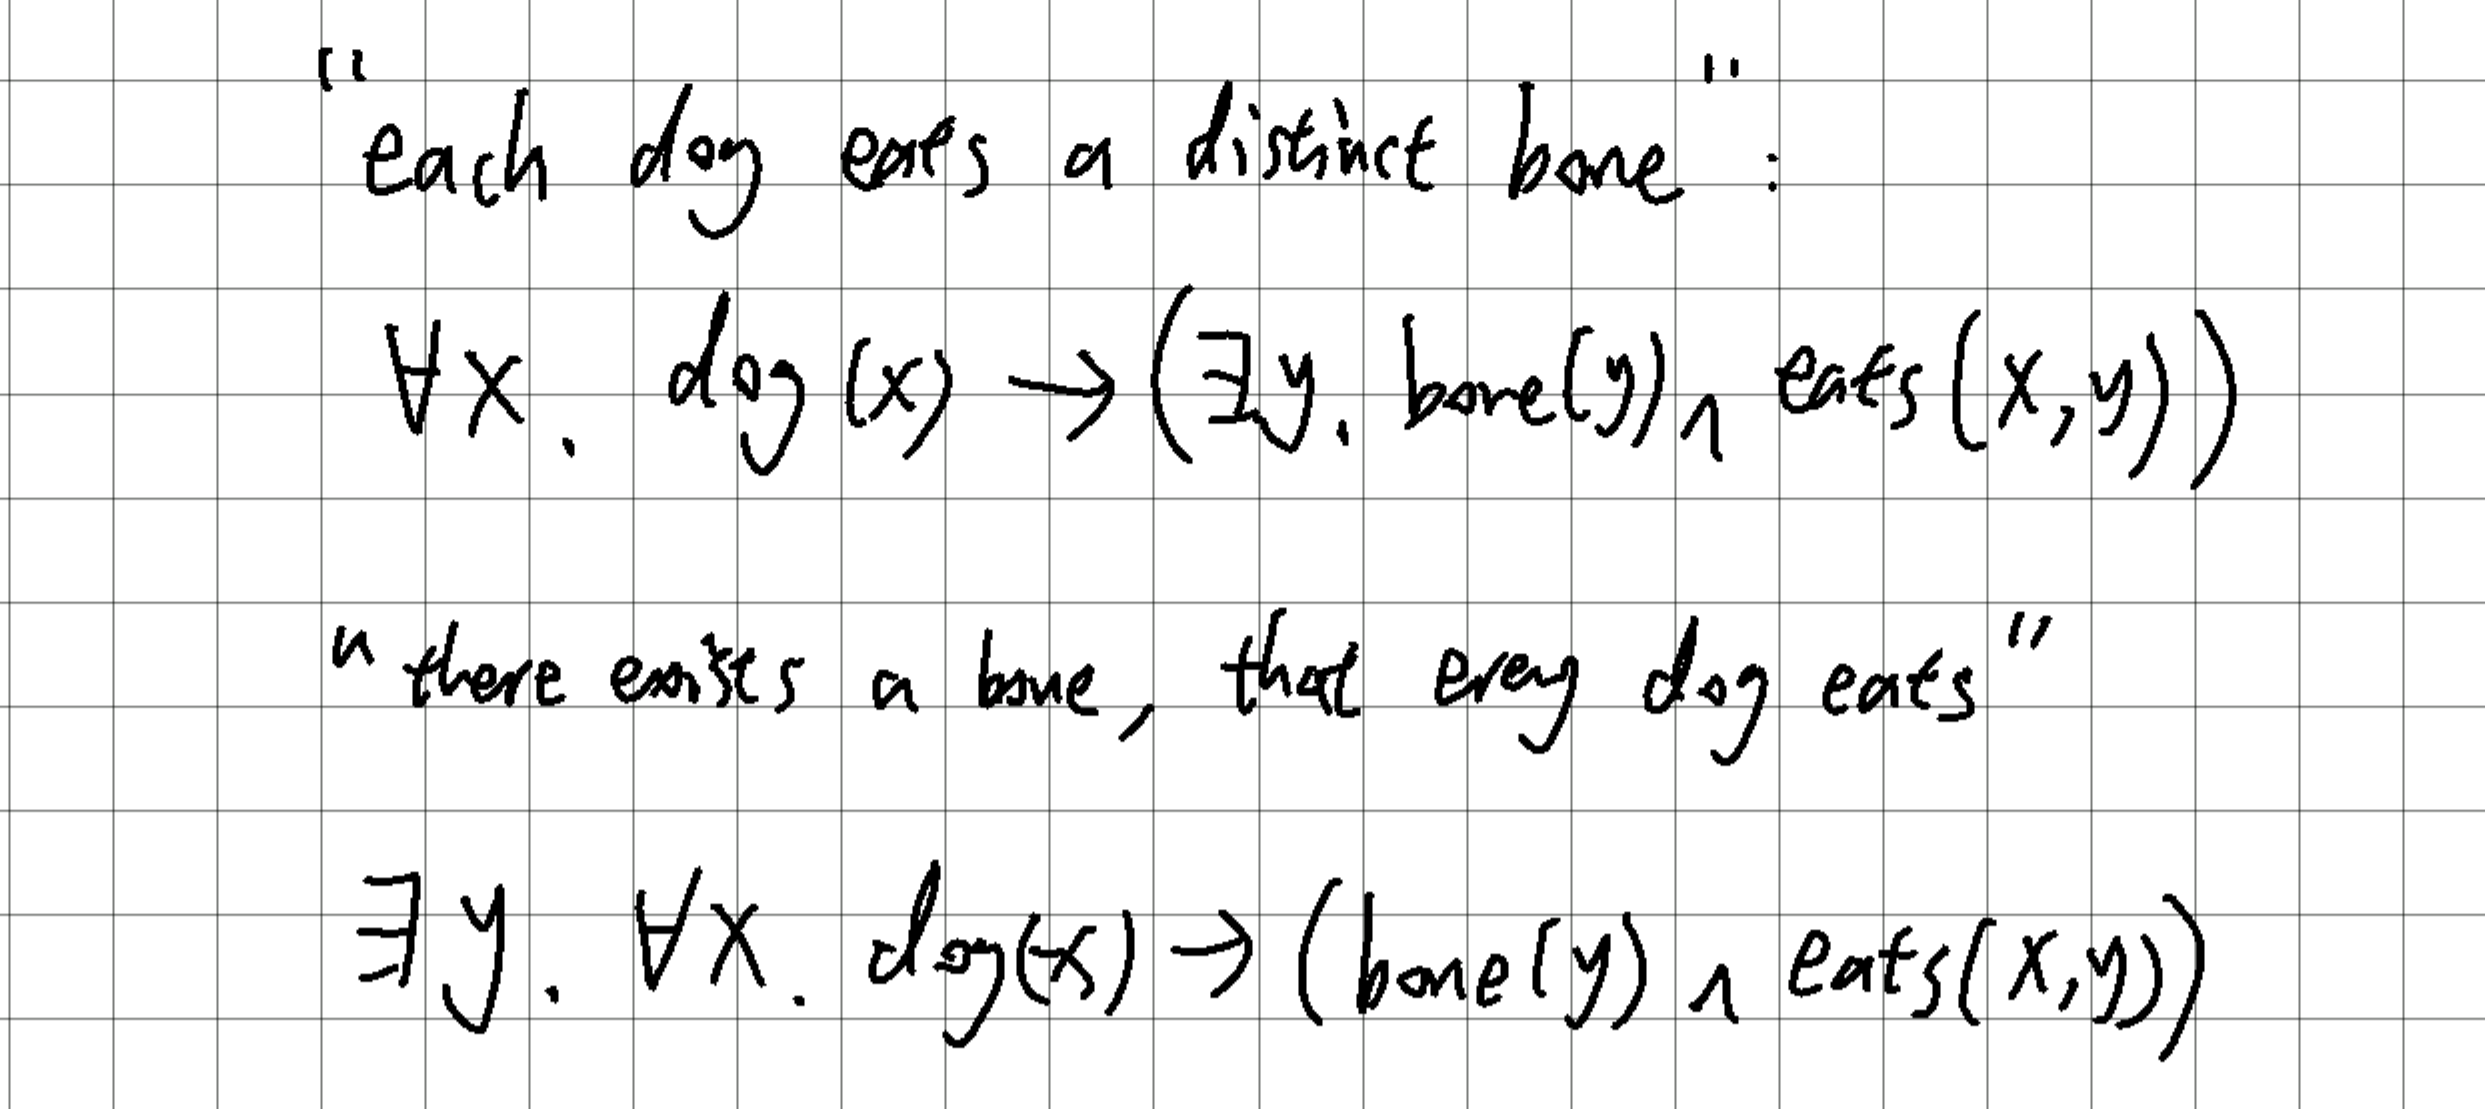
\includegraphics[width=0.7\linewidth]{../disambiguation}
  	\caption{problem 3 (b)}
  	\label{fig:02}
  \end{figure}

\end{document} 
